% !TeX root = ../thesis.tex

\chapter{系统评估}

本章重点介绍在 FPGA 上对系统的构建和评估,实验的目标主要分为以下几个方面:

\begin{itemize}
    \item 验证硬件实现的正确性;
    \item 验证软件实现的正确性;
    \item 验证软硬件协同设计的用户态中断的性能优势;
    \item 分析测试结果与硬件行为间的联系。
\end{itemize}

\section{实验环境}

\begin{figure}
    \centering
    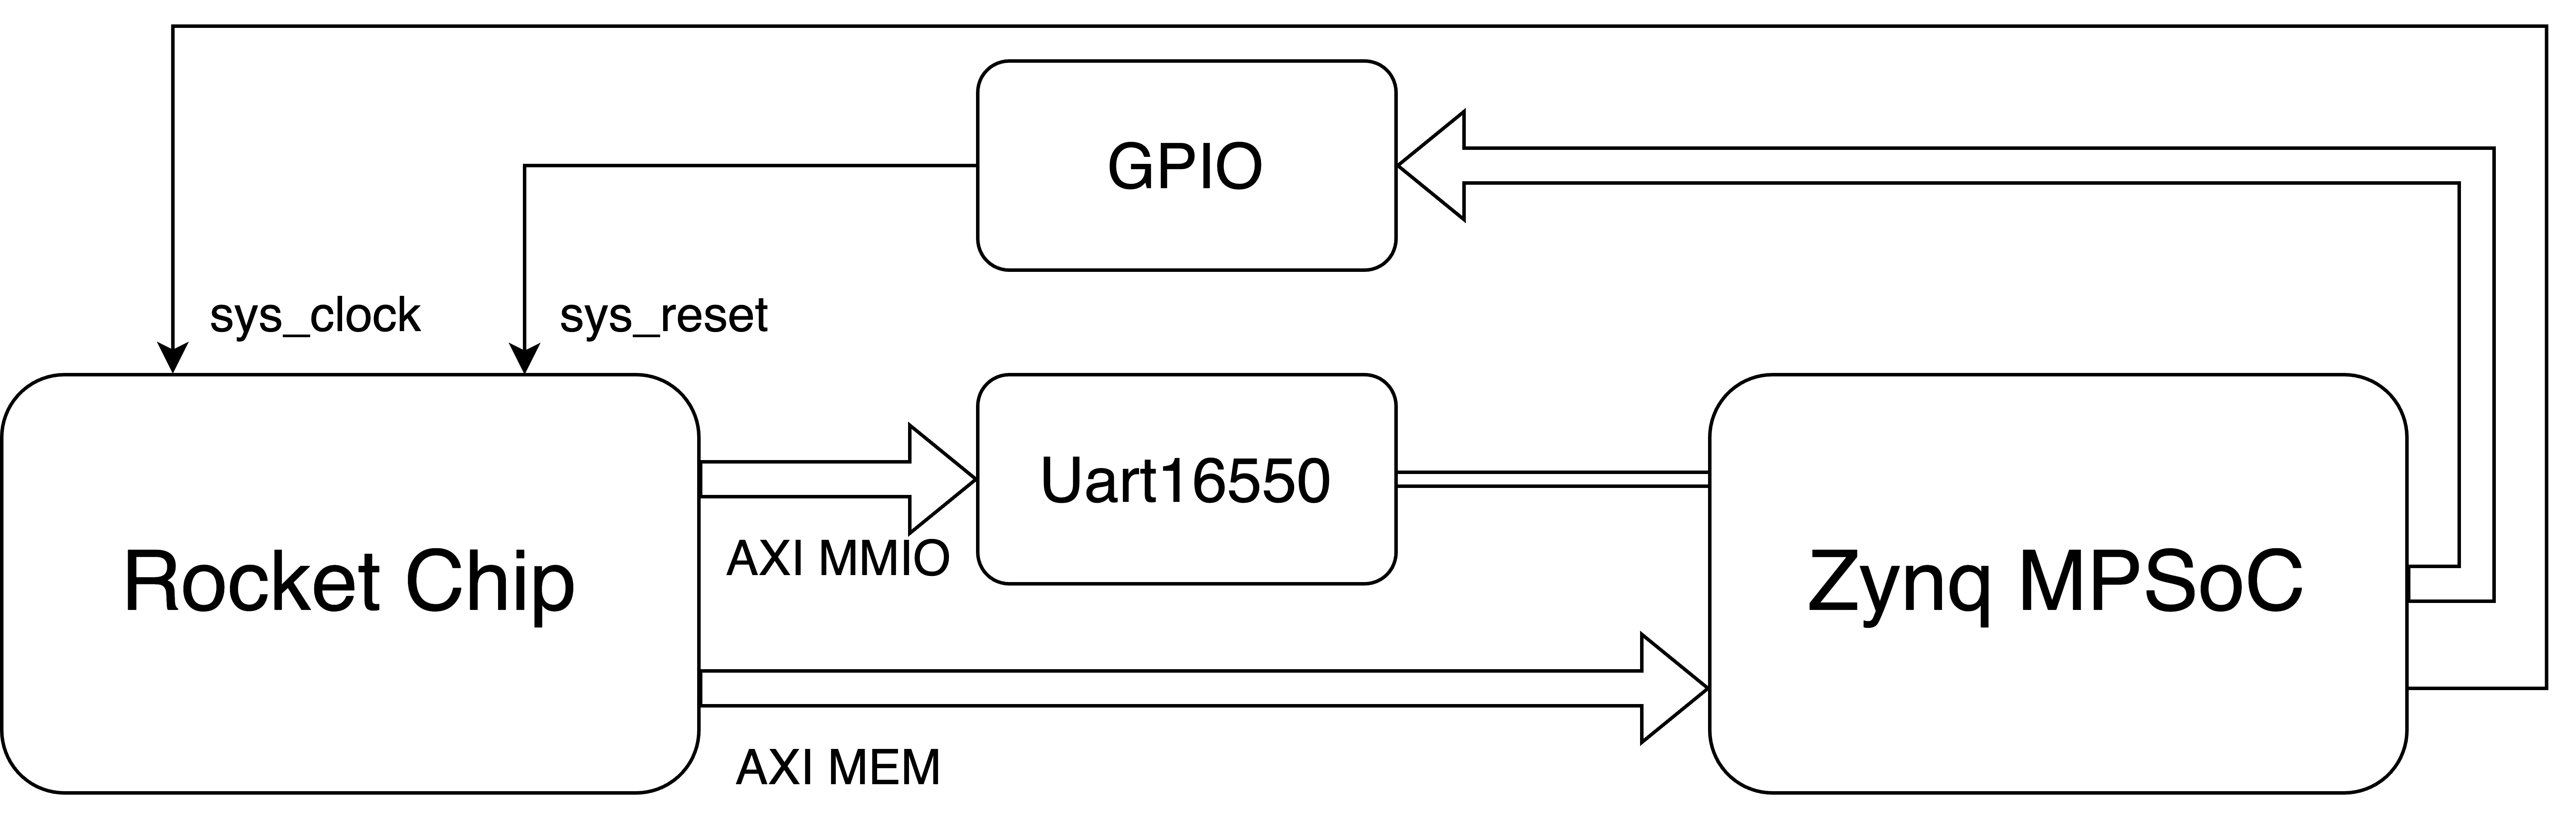
\includegraphics[width=0.8\linewidth]{figures/soc.png}
    \caption{SoC 整体架构}
    \label{fig:soc}
\end{figure}

本文实验主要在 Zynq UltraScale+ MPSoC ZCU102 开发板上开展。ZCU102 分为两个部分,分别为处理器子系统(PS) 和 可编程逻辑(PL) 。PS 提供一款四核 ARM® Cortex®-A53、双核 Cortex-R5F 实时处理器,可以直接对开发板上的资源进行控制;PL 端可以通过 DDR4 组件访问内存资源。

首先,应用 Xilinx 提供的 petalinux SDK 构建在 PS 上运行的 Linux 系统,并挂载 SD 卡作为系统的存储外设。如图 \ref{fig:soc} 所示,引入 AXI GPIO IP 核并在 PS 的设备树给出相关信息,GPIO 的出端口连接到 Rocket Chip 内部,可以在 PS 上操作 /sys/class/gpio/* 来写入这个端口对 Rocket Chip 进行复位。

利用 Rocket Chip 支持的自定义端口和自定义配置参数构建顶层模块。自定义配置包括加入第三章最后一节介绍的 UIPI 协处理器,设置 BootROM 的地址和加载内容。Rocket Chip 顶层模块需要对外暴露两个 AXI master 接口,MEM 端口访问位于 PS 端的 DDR 控制器,MMIO 端口访问 PL 上引入的 Uart16550 IP 核。关于两个端口的地址映射,需要将 Rocket Chip 配置的映射和 Block Design 构建时指定的地址映射相对应。

进一步地,定义系统的顶层模块对 Rocket Chip 顶层模块和 Block Design 模块进一步封装,该模块会对 AXI 接口的位宽进行处理,此外,由于 Rocket Chip 默认看到的内存起始地址为 0x80000000 ,而 Block Deisgn 中 DDR 控制器访问端口的地址映射起始地址为 0 ,需要在模块中对地址高位进行截断。

为了与 Rocket Chip 上运行的系统软件进行交互,引入 Uart16550 IP 核,虽然 Rocket Chip 能够自动生成与内部配置有关的设备树信息,但缺少 PL 额外引入的设备的设备信息,需要手动加入 Uart16550 的设备树节点。

\begin{figure}
    \centering
    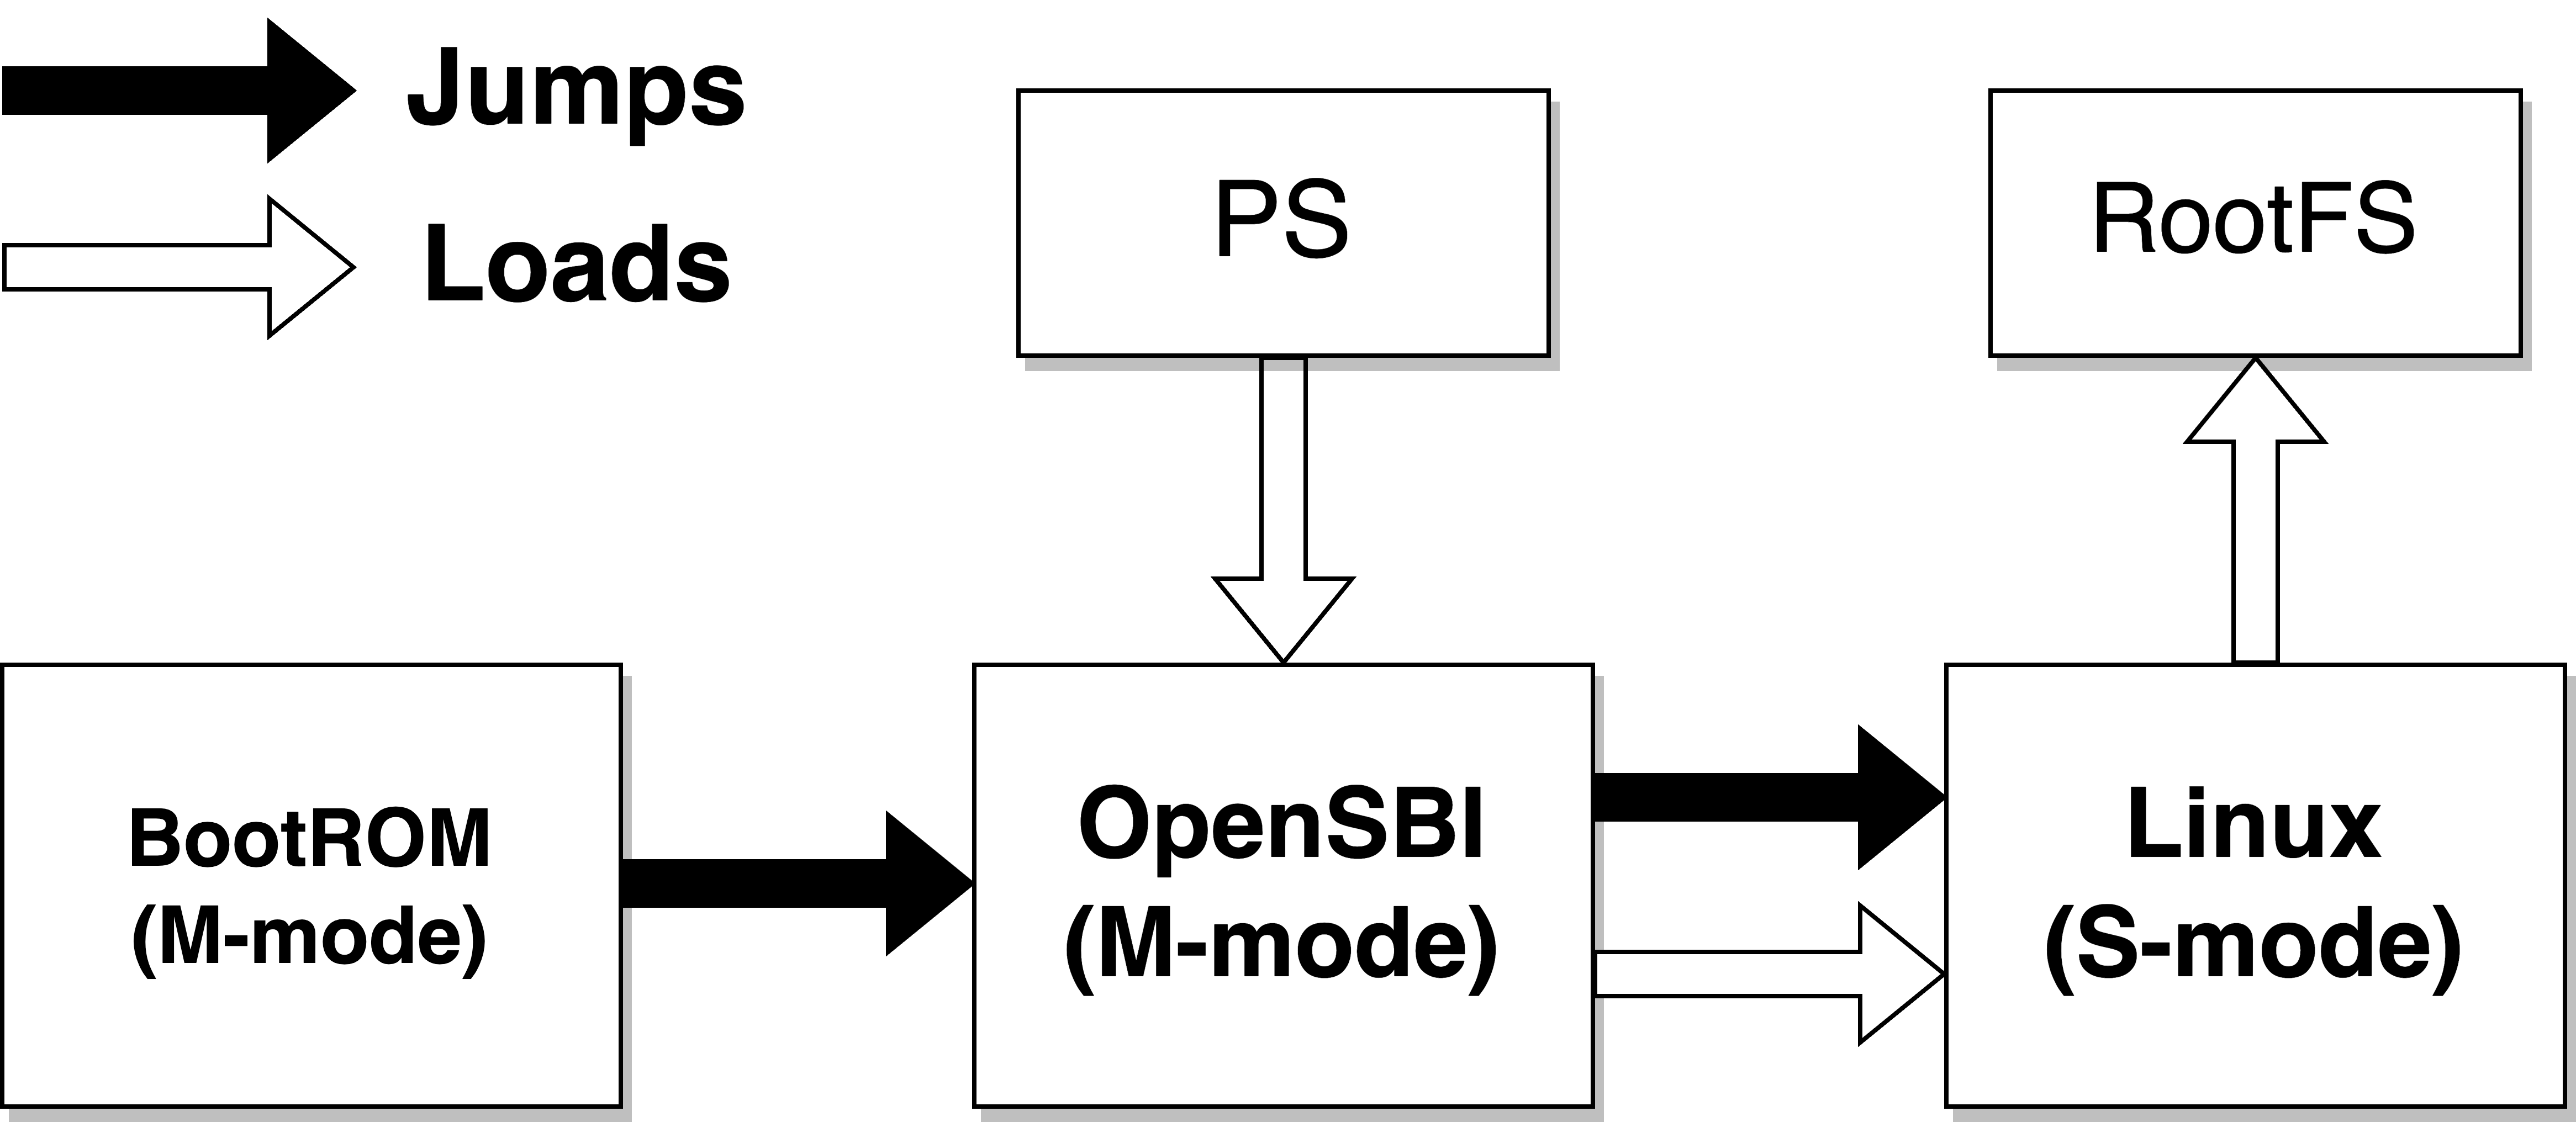
\includegraphics[width=0.8\linewidth]{figures/boot.png}
    \caption{系统软件启动流程}
    \label{fig:boot}
\end{figure}

系统软件的启动流程如图 \ref{fig:boot} 所示。BootROM 为 Rocket Chip 内置的启动代码,在构建时会提前写入到模块中,跳转地址默认为内存的起始地址。

OpenSBI (RISC-V Open Source Supervisor Binary Interface) \cite{opensbi} 是 RISC-V 架构下的 Bootloader,支持通用 SBI 接口,支持 dynamic、jump、payload 三种启动方式。本文的实验采用 payload 启动方式,OpenSBI 镜像会根据 Linux 镜像和设备树的文件位置一起构建。OpenSBI 会在运行时将 Linux 镜像加载到目标地址,并将设备树放在指定的地址。跳转到 Linux 镜像前,OpenSBI 会将核号、设备树地址等信息传递给 Linux 用于 Linux 进一步的初始化。

Buildroot \cite{buildroot} 是一个构建嵌入式 Linux 系统的框架。本文的实验使用 Buildroot 构建根文件系统,并在 Linux 的编译选项中指定文件系统镜像的位置,让 Linux 镜像与文件系统镜像一起构建,并将该文件系统作为 initramfs 。此外,为了让 Linux 在启动时可以打印日志,需要在设备树中添加启动参数指定 earlycons 。

如前文所述,PS 可以对 Rocket Chip 进行复位,在复位前,需要把构建好的 OpenSBI 镜像拷贝到内存中,这部分内存以 reserved-memory 的形式挂载到 PS 的 /dev/mem 文件上,PS 可以直接对该文件进行 mmap 操作完成镜像的写入。

Linux 启动后,可以在主机上连接开发板的串口并看到输出:

\begin{figure}
    \centering
    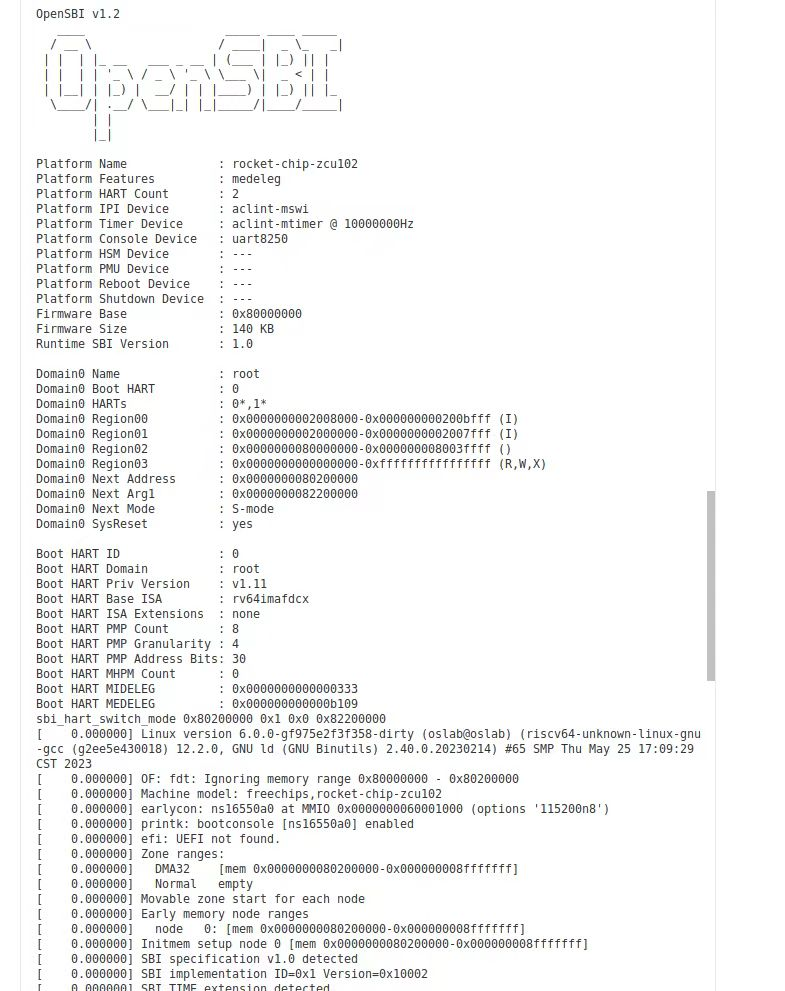
\includegraphics[width=0.9\linewidth]{figures/boot-linux.jpg}
    \caption{启动 Linux}
    \label{fig:boot-linux}
\end{figure}

\section{功能测试}

\subsection{Verilator 仿真测试}

Verilator \cite{verilator} 是一款开源的硬件描述语言仿真器,可以生成 C++仿真代码并在主机上模拟硬件电路的行为。相比于传统的基于事件的仿真器,Verilator 可以更快速、准确地模拟大型电路。
Rocket Chip 集成了 Verilator 仿真器,可以在综合前对 Rocket Chip 进行行为仿真,通过观察 Verilator 生成的波形,可以提早发现并解决硬件逻辑问题,减少硬件调试带来的开销。

riscv-tests \cite{riscvtests} 是一个开源的验证 RISC-V 处理器正确性的测试集,由 RISC-V 基金会开发和维护,包括了 RISC-V 指令集的大部分指令和特性的测试。Rocket Chip 集成该项目并利用 Verilator 对这些测例进行仿真。
基于这一项目,我们实现了多个针对 RISC-V 用户态中断的测例,覆盖了读写 CSR 、中断处理、UIPI 指令等特性。

\subsection{软件接口测试}

\begin{figure}
    \centering
    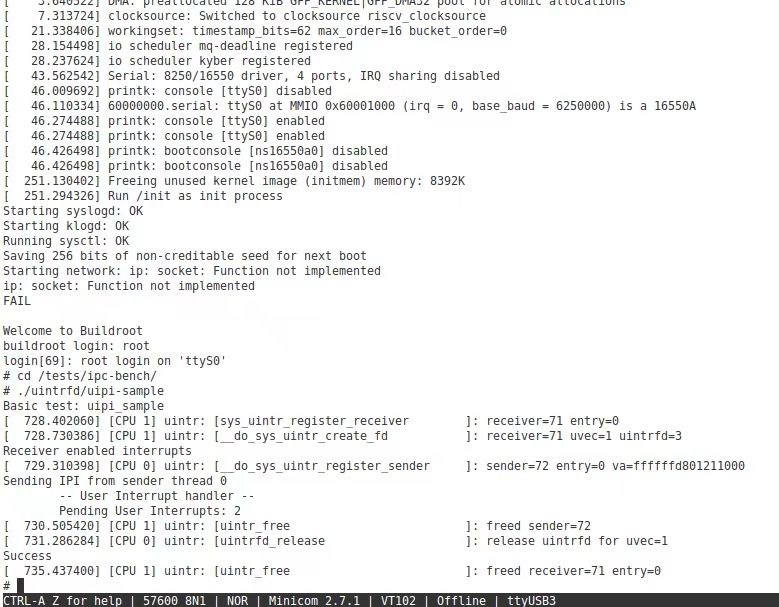
\includegraphics[width=0.8\linewidth]{figures/uipi-sample.jpg}
    \caption{应用程序输出}
    \label{fig:uipi-sample}
\end{figure}

在第四章最后一节中,我们介绍了一个简单的用户态进程间通信程序。分别在 QEMU 模拟器和 Rocket Chip 上启动修改后的 Linux 并运行该程序,可以看到发送方和接收方均正常退出,并释放占用的内核资源,包括文件描述符、发送方状态表等。

\section{性能测试}

ipc-bench \cite{ipcbench} 是一个用来的测试 Linux 和 OS X 操作系统上 IPC 性能的开源项目,包括信号、管道、FIFO、共享内存、TCP 等 IPC 机制。为减少用户程序层面的干扰,对于不同的 IPC 机制采用相同的 Ping-Pong 通信模型,通信的双方会忙等待对方的消息。每个测例会根据配置参数决定某一方收或发的总次数和消息的大小,执行结束后在命令行打印计算得到的性能指标,包括通信的总时间,平均每次通信的时间,吞吐量,标准差。但是实际在统计测试结果时,我们并未完全采纳输出的信息,后续会给出具体的分析。

基于第四章第二节中的库函数,利用 ipc-bench 项目提供的环境,我们实现了针对用户态中断的测试程序。为满足 Ping-Pong 通信模型,该测试程序的通信两端需要同时作为接收方和发送方。在通信开始前,两个线程需要进行一系列的配置,这部分配置不会被包含在总通信时间中。正如上一节所介绍的,我们运行测试的硬件环境是 Rocket Chip,ipc-bench 项目在统计通信时间时,还统计了每次通信的时间来分析标准差等性能指标,需要在每次通信时调用 \texttt{timespec\_get} 函数。这个函数会执行系统调用陷入内核,内核为了获取硬件寄存器中包含的时间信息,执行了 \texttt{rdtime} 这条伪指令,会进一步陷入 OpenSBI 中读取 CLINT 硬件寄存器,整个流程涉及大量的上下文切换,成为了实际的性能瓶颈。对于信号和管道等测例来说可能影响并不是很显著,但是对于 eventfd 和用户态中断等机制来说,每次通信都获取时间会降低测试的准确性。因此在后续的测试中,除用户态中断的测试程序以外,我们也修改了性能对比中用到的测试程序,包括信号、管道和 eventfd ,具体的修改方案为移除每次通信的时间统计,只在通信循环的开始和结束获取时间并计算出通信的总时间。此外,在用户态中断中,消息的大小恒为 1 bit,因此在运行其他测例时,也指定消息大小为 1 bit。

\section{测试结果与分析}

如图是用户态与不同 IPC 机制的性能对比结果。

总体上来看,用户态中断的性能明显优于其他 IPC 机制,说明用户态中断从发出到响应的延迟很低;具体到指令周期,通过 ILA 抓取 Rocket Chip 中的 \texttt{pc} 寄存器,从发送方所在的核执行 \Iuipisend 这条指令开始,到接收方所在的核触发中断处理流程,\texttt{pc} 跳转到 \Rutvec ,总共需要约 100 个时钟周期;根据第四章第二节中对于库函数的介绍,在执行用户指定的中断处理函数之前,需要进行通用寄存器的保存,大概需要约 400 个时钟周期。也就是说从发送方发送用户态中断到接收方响应并开始处理共需要约 500 个时钟周期,这已经远小于应用程序陷入内核再返回的开销了。

相比于其他的 IPC 机制,用户态中断的性能存在一定的波动。在进行软件适配时,需要考虑到接收方是否正在某个核上运行,理想情况下是接收方一直在某个核上运行,用户态中断的延迟可以达到上述的指令周期数;当目标核正处于内核态或运行其他进程时,只有 UINTC 的 Pending Requests 位被写入,UINTC 不会触发用户态中断。当目标接收方被调度时,内核才会在返回用户态前将当前核号写入 UINTC 并将 Active 位置为 1,从而在执行 \Isret 返回用户态的第一条指令触发用户态中断并陷入到用户态中断处理函数中。接收方不在核上运行的流程可以类比用户为某个信号注册处理函数的情况,二者都是经历了\textbf{恢复-陷入-恢复} 的过程,在这种情况下,用户态中断的响应延迟会增加,但一般来说会比信号的处理更快,因为信号处理需要两次切换特权级,而用户态中断只需要一次切换特权级,所以用户态中断的处理相比信号的处理对于页表和缓存系统来说更加友好。时钟中断会导致用户程序陷入到内核,从而导致用户态中断的响应延迟增加,因此用户态中断性能存在一定波动。

在实验的设计中,我们尽可能地减少其他因素对结果的影响,可以将通信总时间与通信次数近似地看成线性关系,从而可以计算出回归方程,其中斜率为单次通信的时间,因为实验开始时要获取时间,且缓存系统也需要预热,所以截距不为 0 。对比单次通信的时间,可以计算出用户态中断相对于其他 IPC 机制的加速比:

